\section{解析と結果}


\begin{figure}
  \centering
  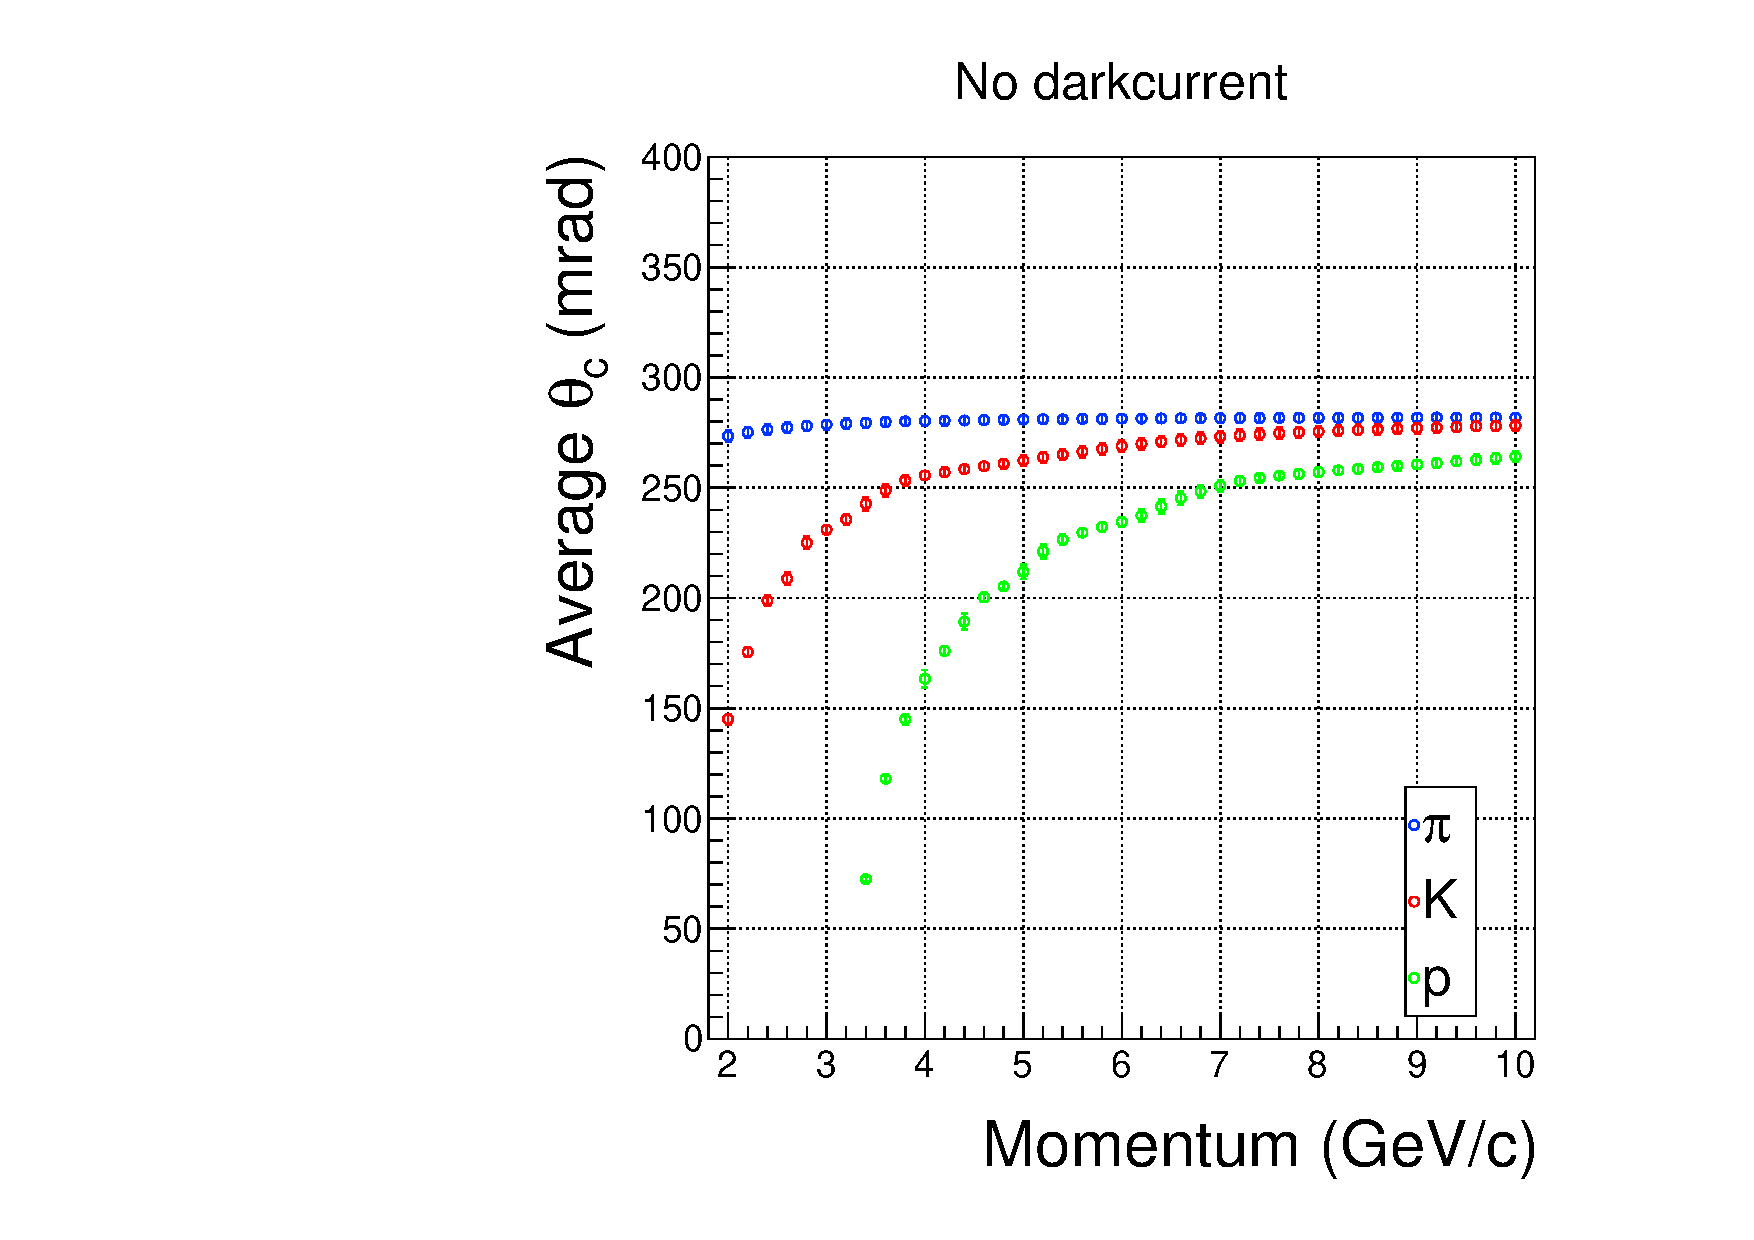
\includegraphics[width=10cm,page=1]{images/chapter4/angleAndMultiGraph.pdf}
  \caption{
    暗電流を考慮しない場合の運動量毎のチェレンコフ角分布。青い点が$\pi$、赤い点がK、緑の点がpを示す。
    エラーバーはチェレンコフ角の分布をガウスフィットした際の$1\sigma$(角度分解能)としている。
  }
  \label{fig:angleMultiGraph1}
\end{figure}